\section{Auswertung}
\subsection{Stabilitätsbedingung}
Zur Überprüfung der Stabilitätsbedingung wurden mehrere Spiegelkombinationen verwendet.
Begonnen wurde mit zwei Spiegeln mit jeweils $R_1 = 1400 \, \text{mm}$.
Für diese Konfiguration konnte eine maximale Resonatorgröße von $L_{Max} = 210 \, \text{cm}$ erreicht werden.

Für die nächste Konfiguration wurde zwei Spiegel mit $R_1 = 1400$ und $R_2 = \infty$ genutzt.
Mit dieser Konfiguraton wurde eine maximale Resonatorgröße von $L_{Max} = 130 \, \text{cm}$ erreicht

\subsection{Polaristaion}
Zur bestimmung der Polaristaion des Lasers wurde ein Polarisationsfilter in den Strahlengang eingebracht. Sodann Wertepaare für
Winkel des Polarisationsfilters und Photostrom aufgenommen werden können. Werden die Messwerte visualisiert ergibt sich \autoref{abb:pol}

\begin{figure}[h]
  \centering
  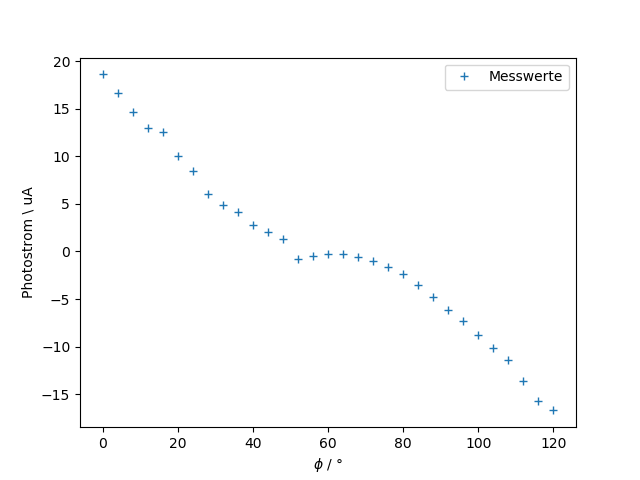
\includegraphics[width=0.75\textwidth]{img/pol.png}
  \caption{Photostrom in Abhängigkeit der Polarisatorachse}.
  \label{abb:pol}
\end{figure}

Es ist zu beobachten, dass der Photostrom für einen eingestellten Winkel des Polarisationsfilters von 60 Grad verschwindet.
Die 0 Grad Linie des Filters steht Horizontal, die Polarisationsachse stehst orthogonal auf dem gemessenen Winkel von 60 Grad.


\subsection{TEM-Mode}
\subsubsection{LP00 - Mode}

Werden die Messwerte zur $LP_{00}$ aufgetragen ergibt sich \autoref{abb:lp00}.


\begin{figure}[h]
  \centering
  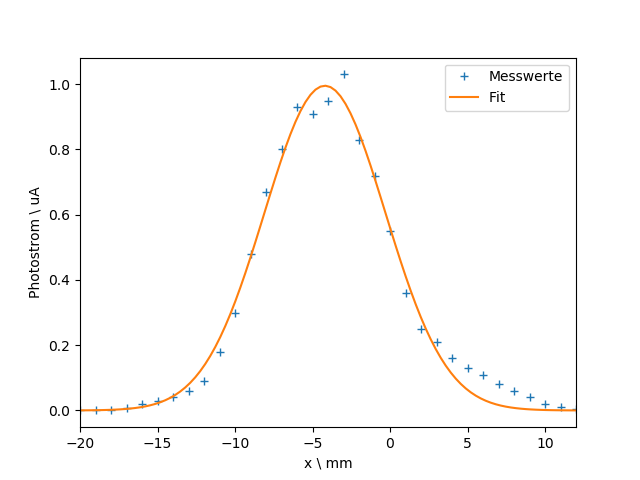
\includegraphics[width=0.75\textwidth]{img/lp00.png}
  \caption{}.
  \label{abb:lp00}
\end{figure}

Eine Ausgleichsrechnung mit 

\begin{equation}
I(r) = I_0 \exp{- \frac{2 (r - \delta r)^2}{w^2}}
\end{equation}

liefert folgende Fit-Parameter

\begin{table}[h]
	\label{tab:lp00}
	\centering
	\begin{tabular}{ccc}
  $I_0$ & $\delta r$ & $w$ \\
  \hline
  1,00 $\pm$ 0,02 & -4,20 $\pm$ 0,09 & 7,8 $\pm$ 0,2 \\
	\end{tabular}
  \caption{Ausgleichsrechnung zur LP00 Mode.}
\end{table}

wobei der Parameter $\delta r$ die Verschiebung der Gauskurve auf der x Achse repräsentiert.

\clearpage

\subsubsection{LP01 - Mode}

Werden die Messwerte zur $LP_{01}$ aufgetragen ergibt sich \autoref{abb:lp01}.

\begin{figure}[h]
  \centering
  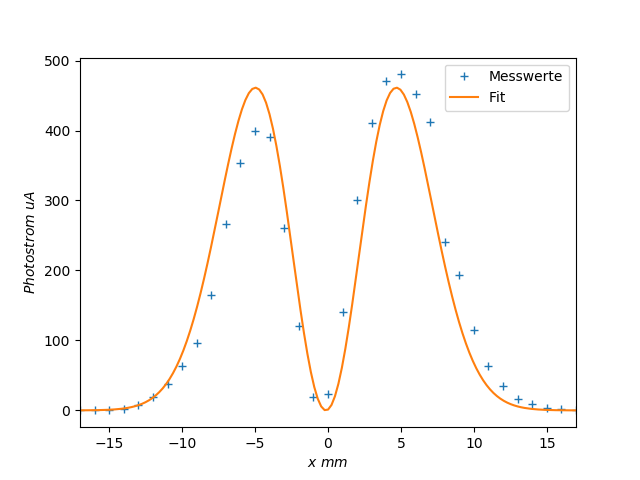
\includegraphics[width=0.75\textwidth]{img/lp01.png}
  \caption{Ausgleichsrechnung bezüglich der LP01 Mode}.
  \label{abb:lp01}
\end{figure}

Eine Ausgleichsrechnung mit

\begin{equation}
I(r) = I_0 (r - \delta r)^{2} \exp{- \frac{2 (r - \delta r)^2}{w^2}}
\end{equation}

liefert folgende Fit-Parameter.

\begin{table}[h]
	\label{tab:lp01}
	\centering
	\begin{tabular}{cccc}
  Mode & $I_0$ & $\delta r$ & $w$ \\
  \hline
  $LP_{01}$ & 54 $\pm$ 4 & -0,1 $\pm$ 0,1 & 9,7 $\pm$ 0,2 \\
	\end{tabular}
  \caption{Ausgleichsrechnung zur LP01 Mode.}
\end{table}

\clearpage

\subsection{longitudinale Mode}

Für die auswertung der longitunalen Mode wurden die enthaltenen Frequenzen im transmittierten Licht mit
einem Frequenzanalysator untersucht. Dabei ist zu beachten, dass diese Frequenzen über

\begin{equation}
f_n = \frac{Nc}{2L}
\end{equation}

mit der Länge des Resonators und der Lichtgeschwindigkeit verknüpft ist.

\begin{figure}[!h]
  \centering
  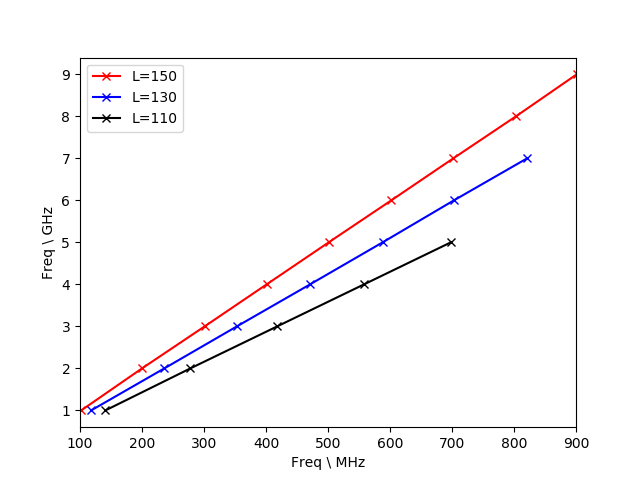
\includegraphics[width=0.75\textwidth]{img/longMode.png}
  \caption{Fequenzen der longitunalen Mode in Abhängigkeit der Resonatorlänge.}
  \label{abb:longMode}
\end{figure}

Aus \autoref{abb:longMode} ist direkt ersichtlich, dass die Steigung der Grade für die verschiedenen
Resonatorlängen proportional zu L ist.

Durch gaußförmige Dopplerverbreiterung der eigentlich scharfen Emissionslinien entsteht eine gaußförmige
Einhüllende über eine gewisse Anzahl von "diskreten" Frequenzkomponenten. Da eine Mindestintensität
für die Verstärkung im Resonator benötigt wird, werden Frequenzkomponenten die 
zu weit vom Linienschwerpunkt des Lasers liegen Unterdrückt.
Somit Läuft der Laser im Multimodenbetrieb, wenn die Breite der Einhüllenden $\Delta f$ größer ist als
der Frequenzabstand $\Delta \phi$ zwischen den Einzelnen Moden.



